% arara: lualatex: { interaction: nonstopmode, synctex: yes }

\documentclass[letterpaper,12pt,oneside,onecolumn]{memoir}

\usepackage{graphicx,epstopdf,amsmath,amssymb,url,booktabs}
\usepackage{microtype,todonotes}
\usepackage[american]{babel}
\usepackage[sf,sc]{titlesec}
\usepackage{tikz}
\usetikzlibrary{shapes,backgrounds}
\usepackage[autostyle]{csquotes}
\clubpenalty = 10000 % Reduce orphans and widows
\widowpenalty = 10000

\usepackage[authordate,url=false,isbn=false,backend=biber]{biblatex-chicago} %Change authordate to notes if desired.
\addbibresource{/Users/rlridenour/Dropbox/bibtex/rlr.bib}


\usepackage{lualatex-math,luatextra}
\usepackage{libertinus}
\usepackage{unicode-math}
\usepackage[unicode=true]{hyperref}

\usepackage{xcolor}
\hypersetup{
    colorlinks,
    linkcolor={red!50!black},
    citecolor={blue!50!black},
    urlcolor={blue!80!black}
}

\title{Pursuing Truth: A Guide to Critical Thinking}
\author{Randy Ridenour}
% \date{}  % Activate to display a given date or no date

\begin{document}


\frontmatter

\begin{titlingpage}
  \maketitle
\end{titlingpage}
  


\tableofcontents*


\chapter{Preface}
\label{chap:preface}

This is a textbook written primarily for my students in PHIL 1502: Critical Thinking, at Oklahoma Baptist University in Shawnee, Oklahoma.

There are many good textbooks for critical thinking on the market today, so why write another one? First, all of those books were written for someone else's course. None cover all of the topics that I would like to cover in class. Second, as I'm sure any student can attest to, textbooks are remarkably expensive, to the point that most of the world's population cannot afford access to good learning material. I'm beginning to think of access to information as a moral issue.  Now, if I could become wealthy by publishing a book on critical thinking, I might be willing to put the ethical considerations aside.\footnote{As a wise man once said, every person has to decide for themselves what level of hypocrisy they're willing to live with.} Since all profit would likely go to the publisher, however, I might as well just give the book away.

Warning: if you are looking for the perfect book on critical thinking, this will not be it. For various reasons, this text is likely to always be a work in progress. I can promise, though, that it will be worth as least as much as you paid for it.

%%% Local Variables:
%%% mode: latex
%%% TeX-master: "ct-text"
%%% End:


\mainmatter


\chapter{Introduction}
\label{chap:intro}

\section{Welcome}
\label{sec:welcome}

We human beings find it very difficult to completely clear our minds. That means you have been thinking of something nearly every waking moment since you began to think. If we assume eight hours of sleep every night, then that comes to just over 7,000,000 minutes of thinking in 20 years. Surely, after that much time spent doing something, you ought to have become pretty good at it. So, why should you consider reading a book or taking a course that claims to teach you how to do something you've been doing for years?

Well, as the old saying goes, I have some good news and some bad news. The bad news is that we're just not very good at thinking carefully. Some things are easy enough for us -- you probably don't have a problem when it comes to deciding whether you should step out in front of a truck. On the other hand, when it comes to difficult, tricky subjects, we're often more likely to come up with wrong answers as right ones.

For example, consider this problem:

\begin{quote}
A ball and bat together cost \$1.10, and the bat costs \$1.00 more than the ball does. How much does the ball cost?
\end{quote}

I'll give you some time to think about your answer, although you shouldn't need much time. So, whenever you're ready, turn the page\ldots

\newpage

Was your answer ten cents? That's the most common answer, but it's also clearly wrong. If the ball costs ten cents, and the bat costs a dollar more than the ball, then the bat costs \$1.10 and the total would be \$1.20. The right answer has to be five cents: \$1.05 + \$.05 = \$1.10. Even though it's not a difficult problem, most people get it wrong.

On the other hand, maybe we get it wrong \emph{because} it's not a difficult
problem. It looks so simple that we answer it without thinking about it.
When we don't reason carefully about a problem, our minds provide us
with an automatic answer. In some situations, the automatic answer
provided by the mind is very likely to be true. In others, it is very
likely to be false.

At this point, you might be asking yourself, \enquote{So what?} What's the worst
that could happen, maybe getting a nickel extra in change when you buy
the ball? This still doesn't justify taking a whole course to learn how
to think better, does it?

Consider one more example:

\begin{quote}


1\% of women at age forty who participate in routine screening have
breast cancer. 80\% of women with breast cancer will get positive
mammographies. 9.6\% of women without breast cancer will also get
positive mammographies. A woman in this age group had a positive
mammography in a routine screening. What is the probability that she
actually has breast cancer?
\end{quote}

Unlike the ball and the bat, being wrong in this case could have drastic
consequences---if the doctor guessed too low, then the patient likely
did not receive the treatment she needed. If the doctor guessed too
high, then the patient may received radical treatments that she didn't
need, unnecessary radiation, chemotherapy, or even a radical mastectomy.

Doctors have to make these diagnoses all the time, so surely they would
be good at correctly estimating the patient's likelihood of having the
disease. Most doctors estimated that, in this problem, the patient's
chances of having breast cancer are somewhere between 70 and 80\%. Only
15\% of doctors surveyed were correct, however. Surprisingly, the right
answer is 7.8\%, a mere one-tenth of the estimates by the medical
professionals.\footnote{That doesn't mean that the test should be ignored. It just means
    that the doctors should not immediately begin dangerous treatments.
    What is warranted is further testing to lessen the chances of a
    false positive.}

So, how does one avoid making such mistakes? The best way is to become a
better critical thinker. You've taken the right initial steps by reading
this book and taking this class.

\section{What is Critical Thinking?}
\label{sec:what-is-ct}



There are probably as many definitions of critical thinking as there
books and articles on the subject. Here is a quick working definition
that will suit our purposes:

\begin{description}
\item[Critical Thinking] Thinking clearly and carefully about what to believe or do in a way that is likely to produce a true belief or right action, if there is one. 
\end{description}





There are a few things to note about this definition. First, critical
thinking is practical. It is designed to produce a particular outcome,
either a belief or an action. The goal is to gain true beliefs while
avoiding false beliefs, or to do right actions and avoid doing wrong
ones. At this point, we don't need to rehash old disputes about the
nature of truth or morality, our ordinary understanding of the two
concepts will be fine.

Second, there is nothing that we can do that guarantees a true
belief---at best, we only get likelihood. Nevertheless, when we use the
tools of critical thinking, we will be more likely to get to the truth
than had we not used those tools.

Third, it is important to note that not every question has an answer
that we can know just by thinking carefully about the problem. There are
some questions that have right answers, but just cannot be known by us.
How many life-supporting planets are there in the universe? We know
there is at least one, but we don't yet have the ability to if there are
any others. There are other questions for which there is no right
answer, at least not in the objective sense. What kind of ice cream is
best? You may have your preference, and I might have a different view.
Is either of us wrong? Don't hold up the line in the ice cream shop
telling yourself, \enquote{I know I like chocolate better than vanilla, but
which one is \emph{really} the best?} There is no best in this case, so order
whatever you want.

This is a classic case of what philosophers call purely subjective. A
subjective truth is one that is dependent on what a person prefers,
thinks, believes, etc. Objective truths are true independently of what
anyone thinks, believes, perceives, etc. Critical thinking won't help us
answer the subjective questions, but we don't really have problems with
those. In those cases, it's good enough just to report how we feel,
since that is what makes those subjective beliefs true. Critical
thinking, however, will help us decide if a question is objective or
subjective, and if objective, if it can be answered.

\section{The Tools of Critical Thinking}
\label{sec:tools-ct}

It's not enough to tell someone to think clearly and carefully---we have
to know what clear and careful thinking, and clear and careful thinkers,
look like. Critical thinking is a skill, and like many other skills, it
involves the skilled use of tools. One set of tools will be no surprise;
they are the tools of logic. Good critical thinkers can

\begin{enumerate}

\item   Identify arguments in propositional and categorical logic
\item   Evaluate arguments using truth tables and Venn diagrams
\item   Use the basic rules of probability, and
\item   Identify common logical fallacies.
\end{enumerate}

Another set of tools has been provided by cognitive psychologists.
Critical thinkers need to understand how the human mind works,
especially the systematic ways that the mind is misled. So, critical
thinkers must

\begin{enumerate}
\item   Understand common cognitive biases,
\item   Be aware of the ways that people try to mislead us,
\item   Know the situations in which we tend to reason badly.
\end{enumerate}

Finally, I think that it's not enough that critical thinkers understand
logic. It's not even enough to understand logic and cognitive
psychology. I think there is a moral, or value component to critical
thinking as well. To become a critical thinker is to become a certain  kind of person, a person of  intellectual virtue. So, we will
discuss the importance and roles of such virtues as

\begin{enumerate}
\item   Open mindedness
\item   Intellectual courage
\item   Intellectual humility
\item   Attentiveness
\item   Fairness
\item   Perseverance
\item   Firmness
\end{enumerate}

So, by the end of this book, and by the end of your course, I hope that
you are well on the road to acquiring these skills. Like any other
skills, they cannot be acquired without practice. You will not become a
perfect critical thinker in a semester, maybe not even over the course
of a lifetime. You can, however, take some significant steps on a
journey that leads to one of the most important destinations ever: the
truth.


%%% Local Variables:
%%% mode: latex
%%% TeX-master: "ct-text"
%%% End:

\part{Logic}


\chapter{Arguments}
\label{chap:arguments}

The fundamental tool of the critical thinker is the argument. For a good example of what we are not talking about, consider a bit from a famous sketch by \emph{Monty Python's Flying Circus} \autocite{Cleese:1980aa}:

\begin{quote}
Man: (Knock)\\
Mr. Vibrating: Come in.\\
Man: Ah, Is this the right room for an argument?\\
Mr. Vibrating: I told you once.\\
Man: No you haven't.\\
Mr. Vibrating: Yes I have.\\
Man: When?\\
Mr. Vibrating: Just now.\\
Man: No you didn't.\\
Mr. Vibrating: Yes I did.\\
Man: You didn't!\\
Mr. Vibrating: I did!\\
Man: You didn't!\\
Mr. Vibrating: I'm telling you I did!\\
Man: You did not!!\\
Mr. Vibrating: Oh, I'm sorry, just one moment. Is this a five minute argument or the full half hour?\\
\end{quote}

\section{Identifying Arguments}
\label{sec:ident-argum}

People often use "argument" to refer to a dispute or quarrel between
people. In critical thinking, an argument is defined as

\begin{description}
\item[Argument] A set of statements, one of which is the conclusion and the others are the premises.
\end{description}



There are three important things to remember here:

\begin{enumerate}
\item Arguments contain statements.
\item They have a conclusion.
\item They have at least one premise
\end{enumerate}

Arguments contain statements, or declarative sentences. Statements,
unlike questions or commands, have a truth value. Statements assert that
the world is a particular way; questions do not. For example, if someone
asked you what you did after dinner yesterday evening, you wouldn't
accuse them of lying. When the world is the way that the statement says
that it is, we say that the statement is true. If the statement is not
true, it is false.

One of the statements in the argument is called the conclusion. The
conclusion is the statement that is intended to be proved. Consider the
following argument:


\begin{quote}
Calculus II will be no harder than Calculus I. Susan did well in
Calculus I. So, Susan should do well in Calculus II.
\end{quote}

Here the conclusion is that Susan should do well in Calculus II. The
other two sentences are premises. Premises are the reasons offered for
believing that the conclusion is true.

\section{Standard Form}
\label{sec:standard-form}

Now, to make the argument easier to evaluate, we will put it into what is called "standard form." To put an argument in standard form, write each premise on a separate, numbered line. Draw a line underneath the last premise, the write the conclusion underneath the line.


\begin{enumerate}
  % \tightlist
\item Calculus II will be no harder than Calculus I.
\item \underline{Susan did well in Calculus I.}
\item [$\therefore$] Susan will do well in Calculus II.
\end{enumerate}

 Now that we have the argument in standard form, we can talk about premise 1, premise 2, and all clearly be referring to the same thing.

\section{Indicator Words}
\label{sec:indicator-words}

Unfortunately, when people present arguments, they rarely put them in standard form. So, we have to decide which statement is intended to be the conclusion, and which are the premises. Don't make the mistake of assuming that the conclusion comes at the end. The conclusion is often at the beginning of the passage, but could even be in the middle. A better way to identify premises and conclusions is to look for indicator words. Indicator words are words that signal that statement following the indicator is a premise or conclusion. The example above used a common indicator word for a conclusion, 'so.' The other common conclusion indicator, as you can probably guess, is 'therefore.' This table lists the indicator words you might encounter.

% Please add the following required packages to your document preamble:
% \usepackage{booktabs}
\begin{table}[]
\begin{tabular}{@{}ll@{}}
Conclusion      & Premise             \\
Therefore       & Since               \\
So              & Because             \\
Thus            & For                 \\
Hence           & Is implied by       \\
Consequently    & For the reason that \\
Implies that    &                     \\
It follows that &                    
\end{tabular}
\end{table}

Each argument will likely use only one indicator word or phrase. When the conlusion is at the end, it will generally be preceded by a conclusion indicator. Everything else, then, is a premise. When the conclusion comes at the beginning, the next sentence will usually be introduced by a premise indicator. All of the following sentences will also be premises.

For example, here's our previous argument rewritten to use a premise indicator:

\begin{quote}
Susan should do well in Calculus II, because Calculus II will be no harder than Calculus I, and Susan did well in Calculus I.
\end{quote}

Sometimes, an argument will contain no indicator words at all. In that case, the best thing to do is to determine which of the premises would logically follow from the others. If there is one, then it is the conclusion. Here is an example:

\begin{quote}
Spot is a mammal. All dogs are mammals, and Spot is a dog.
\end{quote}

The first sentence logically follows from the others, so it is the conclusion. When using this method, we are forced to assume that the person giving the argument is rational and logical, which might not be true.

\section{Non-Arguments}
\label{sec:non-arguments}

One thing that complicates our task of identifying arguments is that there are many passages that, although they look like arguments, are not arguments. The most common types are:

\begin{enumerate}
\item Explanations
\item Mere asssertions
\item Conditional statements
\item Loosely connected statements
\end{enumerate}

Explanations can be tricky, because they often use one of our indicator words. Consider this passage:

\begin{quote}
Abraham Lincoln died because he was shot.
\end{quote}

If this were an argument, then the conclusion would be that Abraham Lincoln died, since the other statement is introduced by a premise indicator. If this is an argument, though, it's a strange one. Do you really think that someone would be trying to prove that Abraham Lincoln died? Surely everyone knows that he is dead. On the other hand, there might be people who don't know how he died. This passage does not attempt to prove that something is true, but instead attempts to explain why it is true. To determine if a passage is an explanation or an argument, first find the statement that looks like the conclusion. Next, ask yourself if everyone likely already believes that statement to be true. If the answer to that question is yes, then the passage is an explanation.

Mere assertions are obviously not arguments. If a professor tells you simply that you will not get an A in her course this semester, she has not given you an argument. This is because she hasn't given you any reasons to believe that the statement is true. If there are no premises, then there is no argument.

Conditional statements are sentences that have the form \enquote{If\ldots, then\ldots} A conditional statement asserts that \emph{if} something is true, then something else would be true also. For example, imagine you are told, \enquote{If you have the winning lottery ticket, then you will win ten million dollars.} What is being claimed to be true, that you have the winning lottery ticket, or that you will win ten million dollars? Neither. The only thing claimed is the entire conditional. Conditionals can be premises, and they can be conclusions. They can be parts of arguments, but that cannot, on their own, be arguments themselves.

Finally, consider this passage:

\begin{quote}
I woke up this morning, then took a shower and got dressed. After breakfast, I worked on chapter 2 of the critical thinking text. I then took a break and drank some more coffee\ldots.
\end{quote}

This might be a description of my day, but it's not an argument. There's nothing in the passage that plays the role of a premise or a conclusion. The passage doesn't attempt to prove anything. Remember that arguments need a conclusion, there must be something that is the statement to be proved. Lacking that, it simply isn't an argument, no matter how much it looks like one.

\section{Evaluating Arguments}
\label{sec:evaluating-arguments}

The first step in evaluating an argument is to determine what kind of argument it is. We initially categorize arguments as either deductive or inductive, defined roughly in terms of their goals. In deductive arguments, the truth of the premises is intended to absolutely establish the truth of the conclusion. For inductive arguments, the truth of the premises is only intended to establish the probable truth of the conclusion. We'll focus on deductive arguments first, then examine inductive arguments in later chapters.

Once we have established that an argument is deductive, we then ask if it is valid. To say that an argument is valid is to claim that there is a very special logical relationship between the premises and the conclusion, such that if the premises are true, then the conclusion must also be true. Another way to state this is

\begin{description}
\item [Valid] An argument is valid if and only if it is impossible for the premises to be true and the conclusion false.
\item [Invalid] An argument is invalid if and only if it is not valid.
\end{description}

Note that claiming that an argument is valid is not the same as claiming that it has a true conclusion, nor is it to claim that the argument has true premises. Claiming that an argument is valid is claiming nothing more that the premises, \emph{if they were true}, would be enough to make the conclusion true. For example, is the following argument valid or not?


\begin{enumerate}
\item If pigs fly, then an increase in the minimum wage will be approved next term.
\item \underline{Pigs fly.}
\item [$\therefore$] An increase in the minimum wage will be approved next term.
\end{enumerate}


The argument is indeed valid. If the two premises were true, then the
conclusion would have to be true also. What about this argument?

\begin{enumerate}
  % \tightlist
\item All dogs are mammals 
\item \underline{Spot is a mammal.}
\item [$\therefore$] Spot is a dog.
\end{enumerate}

In this case, both of the premises are true and the conclusion is true. The question to ask, though, is whether the premises absolutely guarantee that the conclusion is true. The answer here is no. The two premises could be true and the conclusion false if Spot were a cat, whale, etc.

Neither of these arguments are good. The second fails because it is invalid. The two premises don't prove that the conclusion is true. The first argument is valid, however. So, the premises would prove that the conclusion is true, \emph{if those premises were themselves true}. Unfortunately, (or fortunately, I guess, considering what would be dropping from the sky) pigs don't fly.

These examples give us two important ways that deductive arguments can fail. The can fail because they are invalid, or because they have at least one false premise. Of course, these are not mutually exclusive, an argument can be both invalid and have a false premise.

If the argument is valid, and has all true premises, then it is a sound argument. Sound arguments always have true conclusions.


\begin{description}
\item[Sound] A deductively valid argument with all true premises.
\end{description}

Inductive arguments are never valid, since the premises only establish the probable truth of the conclusion. So, we evaluate inductive arguments according to their strength. A strong inductive argument is one in which the truth of the premises really do make the conclusion probably true. An argument is weak if the truth of the premises fail to establish the probable truth of the conclusion.

There is a significant difference between valid/invalid and strong/weak. If an argument is not valid, then it is invalid. The two categories are mutually exclusive and exhaustive. There can be no such thing as an argument being more valid than another valid argument. Validity is all or nothing. Inductive strength, however, is on a continuum. A strong inductive argument can be made stronger with the addition of another premise. More evidence can raise the probability of the conclusion. A valid argument cannot be made more valid with an additional premise. Why not? If the argument is valid, then the premises were enough to absolutely guarantee the truth of the conclusion. Adding another premise won't give any more guarantee of truth than was already there. If it could, then the guarantee wasn't absolute before, and the original argument wasn't valid in the first place.

\section{Counterexamples}
\label{sec:counterexamples}

One way to prove an argument to be invalid is to use a counterexample. A counterexample is a consistent story in which the premises are true and the conclusion false. Consider the argument above:

\begin{enumerate}
  % \tightlist
\item All dogs are mammals
\item \underline{Spot is a mammal.}
\item [$\therefore$] Spot is a dog.
\end{enumerate}

By pointing out that Spot could have been a cat, I have told a story in
which the premises are true, but the conclusion is false.

Here's another one:

\begin{enumerate}
  % \tightlist
\item If it is raining, then the sidewalks are wet.
\item \underline{The sidewalks are wet.}
\item [$\therefore$] It is raining.
\end{enumerate}

The sprinklers might have been on. If so, then the sidewalks would be wet, even if it weren't raining.

Counterexamples can be very useful for demonstrating invalidity. Keep in mind, though, that validity can never be proved with the counterexample method. If the argument is valid, then it will be impossible to give a counterexample to it. If you can't come up with a counterexample, however, that does not prove the argument to be valid. It may only mean that you're not creative enough.

\section{Review}
\label{sec:arg-review}



\begin{enumerate}

\item An \textbf{argument} is a set of statements; one is the conclusion, the rest are premises. 
\item The \textbf{conclusion} is the statement that the argument is trying to prove. 
\item The \textbf{premises} are the reasons offered for believing the
  conclusion to be true. 
\item Explanations, conditional sentences, and mere assertions are not arguments. 
\item \textbf{Deductive} reasoning attempts to absolutely guarantee the truth of the conclusion. 
\item \textbf{Inductive} reasoning attempts to show that the conclusion is probably true. 
\item In a \textbf{valid} argument, it is impossible for the premises to be true and the conclusion false. 
\item In an \textbf{invalid} argument, it is possible for the premises to be true and the conclusion false. 
\item A \textbf{sound} argument is valid and has all true premises. 
\item An inductively \textbf{strong} argument is one in which the truth of the premises makes the the truth of the conclusion probable. 
\item An inductively \textbf{weak} argument is one in which the truth of the premises do not make the conclusion probably true. 
\item A \textbf{counterexample} is a consistent story in which the premises of an argument are true and the conclusion is false. Counterexamples can be used to prove that arguments are deductively invalid
\end{enumerate}



%%% Local Variables:
%%% mode: latex
%%% TeX-master: "ct-text"
%%% End:

\chapter{Categorical Logic}
\label{chap:categorical}




Now we turn to some structured logic systems. The first, categorical logic, is one of the oldest. It dates back at least to Aristotle (384--322 BCE). Categorical logic is a fairly simple logic of categories or classes. A class is a group of things that we designate with a common noun: students, teachers, dogs, politicians, etc. Each sentence will use two different classes. One is the subject class, and the other is the predicate class. In this logic, we can say something about all members of a class, called a universal sentence, or we can say something about some members of a class, called a particular sentence. We can also make a positive claim, called an affirmation, or we can make a negative claim, called a negation.

With these two distinctions, universal/particular and affirnation/negation, we can make four kinds of sentences. S and P stand for the subject class and the predicate class, respectively.

\begin{description}
\item[A]: All S are P (universal affirmation)
\item[E]: No S are P (universal negation)
\item[I]: Some S are P (particular affirmation)
\item[O]: Some S are not P (particular negation)\footnote{The letters A, E, I, and O, are thought to come from the first two vowels of the Latin words \emph{affirmo} and \emph{nego}, meaning \enquote{I affirm} and \enquote{I deny.}
} 
\end{description}

Here are some examples of categorical statements, some true and some false.

\begin{enumerate}
\item All dogs are mammals.
\item All mammals are dogs.
\item No reptiles are dogs.
\item No politicians are honest people.
\item Some politicians are honest people.
\item Some cats are amphibians.
\item Some dogs are not beagles.
\item Some beagles are not dogs.
\end{enumerate}

Look at the sentences carefully. You should be able to tell that the odd-numbered ones are true and the even-numbered ones are false.

\section{The Square of Opposition}
\label{sec:square-opposition}

We can visualize interesting logical relationships between these four types of sentences with something called \enquote{The Square of Opposition.}

The first step is to place the sentence types in the corners of an imaginary square. A is at the upper left; E, the upper right; I, the lower left, and O, the lower right. Next, draw arrows on the diagonals, pointing to the sentences in the corners. Then, draw an arrow between the two at the top, and another one between the two at the bottom. Finally, draw an arrow on each side, going from top to bottom. When finished, you should have something like this:

% INSERT DIAGRAM OF SQUARE OF OPPOSITION HERE

\medskip
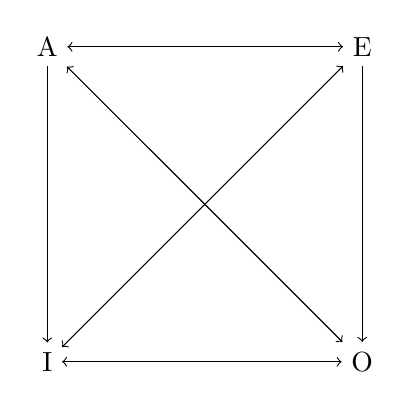
\begin{tikzpicture}
  \node(A) at (0,0) {A};
  \node(E) at (4,0) {E};
  \node(I) at (0,-4) {I};
  \node(O) at (4,-4) {O};
  \draw[<->] (A) -- (E);
  \draw[<->] (I) -- (O);
  \draw[<->] (A) -- (O);
  \draw[<->] (E) -- (I);
  \draw[->] (A) -- (I);
  \draw[->] (E) -- (O);
\end{tikzpicture}

The next step is to note the relationship between the diagonals. The diagonals are contradictories, meaning they always have opposite truth values. They can't both be true, and they also can't both be false.  If the A sentence is true, the O sentence must be false---if it is true that all dogs are mammals, it cannot be true that some dogs are not mammals. If the O sentence is true, then the A sentence must be false. It is the same for the E and the I. 

\medskip
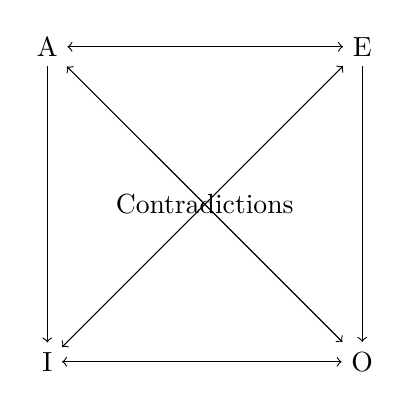
\begin{tikzpicture}
  \node(A) at (0,0) {A};
  \node(E) at (4,0) {E};
  \node(I) at (0,-4) {I};
  \node(O) at (4,-4) {O};
  \draw[<->] (A) -- (E);
  \draw[<->] (I) -- (O);
  \draw[<->] (A) -- (O) node[pos=0.5]{Contradictions};
  \draw[<->] (E) -- (I);
  \draw[->] (A) -- (I);
  \draw[->] (E) -- (O);
  % \draw (-0.5,0) node[left]{Altern};
  % \draw (4.5,0) node[right]{Altern};
  % \draw (-0.5,-4) node[left]{Sub-altern};
  % \draw (4.5,-4) node[right]{Sub-altern};
\end{tikzpicture}

Next, note the relationship between the A sentences and the E sentences, called contraries. Like the contradictories, they cannot both be true. Unlike the contradictories, they can both be false. If it's true that all critical thinking students are good students, then it must be false that no critical thinking students are good students. If it's false that all critical thinking students are good students, then it can be false that critical thinking students are good students. In fact, they are both false, because some critical thinking students are good and others are not. 

\medskip
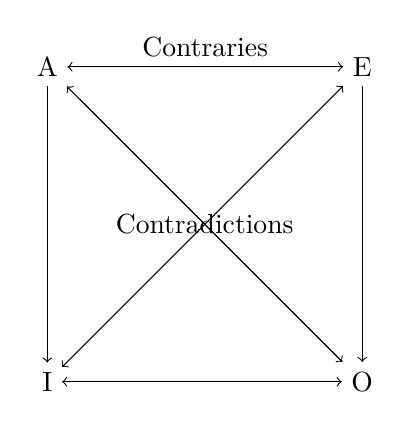
\begin{tikzpicture}
  \node(A) at (0,0) {A};
  \node(E) at (4,0) {E};
  \node(I) at (0,-4) {I};
  \node(O) at (4,-4) {O};
  \draw[<->] (A) -- (E) node[pos=0.5,anchor=south]{Contraries};
  \draw[<->] (I) -- (O);
  \draw[<->] (A) -- (O) node[pos=0.5]{Contradictions};
  \draw[<->] (E) -- (I);
  \draw[->] (A) -- (I);
  \draw[->] (E) -- (O);
  % \draw (-0.5,0) node[left]{Altern};
  % \draw (4.5,0) node[right]{Altern};
  % \draw (-0.5,-4) node[left]{Sub-altern};
  % \draw (4.5,-4) node[right]{Sub-altern};
\end{tikzpicture}

At the bottom, we have sub-contraries. They can both be true, but cannot both be false.

\medskip
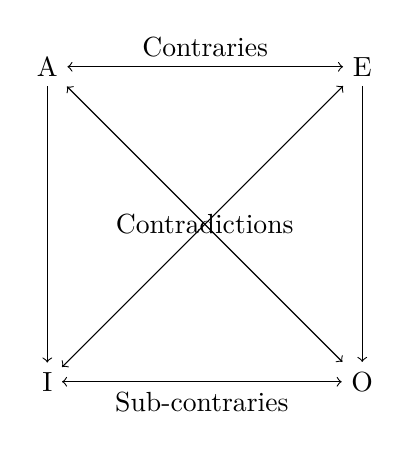
\begin{tikzpicture}
  \node(A) at (0,0) {A};
  \node(E) at (4,0) {E};
  \node(I) at (0,-4) {I};
  \node(O) at (4,-4) {O};
  \draw[<->] (A) -- (E) node[pos=0.5,anchor=south]{Contraries};
  \draw[<->] (I) -- (O)node[pos=0.5,anchor=north]{Sub-contraries};
  \draw[<->] (A) -- (O) node[pos=0.5]{Contradictions};
  \draw[<->] (E) -- (I);
  \draw[->] (A) -- (I);
  \draw[->] (E) -- (O);
  % \draw (-0.5,0) node[left]{Altern};
  % \draw (4.5,0) node[right]{Altern};
  % \draw (-0.5,-4) node[left]{Sub-altern};
  % \draw (4.5,-4) node[right]{Sub-altern};
\end{tikzpicture}

Finally, we have the relationship between the top level sentences and the bottom level sentences on the same side. This is called alternation. The universal is called the superaltern and the particular is called the subaltern. If the superaltern is true, then the subaltern must also be true. If the superaltern is false, then the subaltern can be either true or false. If the subaltern is false, then the superaltern must be false. If the subaltern is true, then the superaltern can be either true or false. It is easy to remember this way: truth goes down, falsity goes up.

\medskip
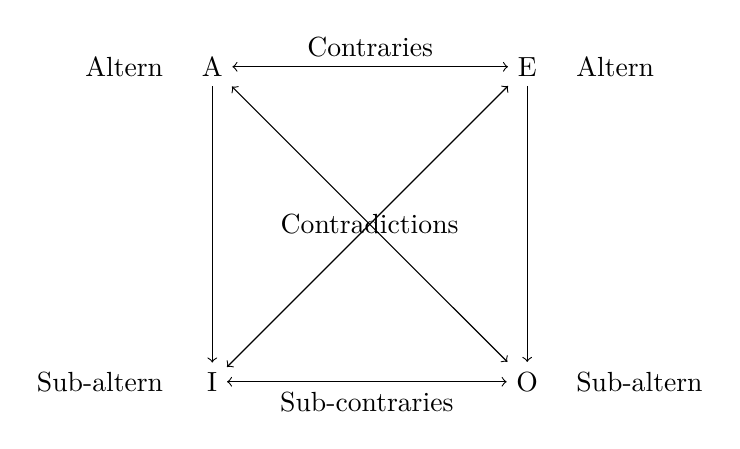
\begin{tikzpicture}
  \node(A) at (0,0) {A};
  \node(E) at (4,0) {E};
  \node(I) at (0,-4) {I};
  \node(O) at (4,-4) {O};
  \draw[<->] (A) -- (E) node[pos=0.5,anchor=south]{Contraries};
  \draw[<->] (I) -- (O)node[pos=0.5,anchor=north]{Sub-contraries};
  \draw[<->] (A) -- (O) node[pos=0.5]{Contradictions};
  \draw[<->] (E) -- (I);
  \draw[->] (A) -- (I);
  \draw[->] (E) -- (O);
  \draw (-0.5,0) node[left]{Altern};
  \draw (4.5,0) node[right]{Altern};
  \draw (-0.5,-4) node[left]{Sub-altern};
  \draw (4.5,-4) node[right]{Sub-altern};
\end{tikzpicture}

\section{Diagramming Sentences}
\label{sec:diagramming-sentences}



We diagram sentences and arguments in categorical logic using Venn diagrams. You've probably used these in a math class at some time. Before we can use these to evaluate arguments in categorical logic, we first have to learn how to diagram individual sentences.

The first step is to draw two interlocking circles. Label the left circle with an \enquote{S} and the right circle with \enquote{P}---standing for the subject term and predicate term, respectively.

\def\sub{(0,0) circle (1.5cm)}
\def\mid{(-60:2cm) circle (1.5cm)}
\def\pred{(0:2cm) circle (1.5cm)}

\medskip
\begin{tikzpicture}[thick,scale=1, every node/.style={transform shape}]
  \begin{scope}
    % A-Sentences

    % \begin{scope}[even odd rule]% Shade S without P
    %   \clip \pred (-1.5,-1.5) rectangle (1.5,1.5);
    %   \fill[gray] \sub;
    % \end{scope}

    % \begin{scope}[even odd rule]% Shade S without M
    %   \clip \mid (-1.5,-1.5) rectangle (1.5,1.5);
    %   \fill[gray] \sub;
    % \end{scope}

    % \begin{scope}[even odd rule]% Shade M without S
    %   \clip \sub (-0.5,-3.3) rectangle (2.5,0);
    %   \fill[gray] \mid;
    % \end{scope}

    % \begin{scope}[even odd rule]% Shade M without P
    %   \clip \pred (-0.5,-3.3) rectangle (2.5,0);
    %   \fill[gray] \mid;
    % \end{scope}

    % \begin{scope}[even odd rule]% Shade P without M
    %   \clip \mid (-0,-1.5) rectangle (3.5,1.5);
    %   \fill[gray] \pred;
    % \end{scope}

    % \begin{scope}[even odd rule]% Shade P without S
    %   \clip \sub (0,-1.5) rectangle (3.5,1.5);
    %   \fill[gray] \pred;
    % \end{scope}

    % E Sentences

    % \begin{scope} %Shade intersection of S and P
    %   \clip \pred;
    %   \fill[gray] \sub;
    % \end{scope}

    % \begin{scope} %Shade intersection of S and M
    %   \clip \mid;
    %   \fill[gray] \sub;
    % \end{scope}

    % \begin{scope} %Shade intersection of M and P
    %   \clip \pred;
    %   \fill[gray] \mid;
    % \end{scope}

    % Mark I and O Sentences

    % \draw (-0.5,0.3) node {1};
    % \draw (1,0.3) node {2};
    % \draw (2.5,0.3) node {3};
    % \draw (0.2,-0.9) node {4};
    % \draw (1,-0.6) node {5};
    % \draw (1.8,-0.9) node {6};
    % \draw (1,-2) node {7};

    % Label Circles

    \draw (-2,-0) node {$S$};
    % \draw (1,-4) node {$M$};
    \draw (4,0) node {$P$};

    % Draw Circles

    \draw \sub;
    \draw \pred;
    % \draw \mid;
  \end{scope}

\end{tikzpicture}

\subsection{A-Sentences}

Remember that the A-sentence has the form All S are P. That means that everything that is in the S circle must also be in the P circle. To diagram this, we shade the region of the S circle that is not contained in the P circle. If a region is shaded, that means that nothing is in that region.



\medskip
\begin{tikzpicture}[thick,scale=1, every node/.style={transform shape}]
  \begin{scope}
    % A-Sentences

    \begin{scope}[even odd rule]% Shade S without P
      \clip \pred (-1.5,-1.5) rectangle (1.5,1.5);
      \fill[gray] \sub;
    \end{scope}

    % \begin{scope}[even odd rule]% Shade S without M
    %   \clip \mid (-1.5,-1.5) rectangle (1.5,1.5);
    %   \fill[gray] \sub;
    % \end{scope}

    % \begin{scope}[even odd rule]% Shade M without S
    %   \clip \sub (-0.5,-3.3) rectangle (2.5,0);
    %   \fill[gray] \mid;
    % \end{scope}

    % \begin{scope}[even odd rule]% Shade M without P
    %   \clip \pred (-0.5,-3.3) rectangle (2.5,0);
    %   \fill[gray] \mid;
    % \end{scope}

    % \begin{scope}[even odd rule]% Shade P without M
    %   \clip \mid (-0,-1.5) rectangle (3.5,1.5);
    %   \fill[gray] \pred;
    % \end{scope}

    % \begin{scope}[even odd rule]% Shade P without S
    %   \clip \sub (0,-1.5) rectangle (3.5,1.5);
    %   \fill[gray] \pred;
    % \end{scope}

    % E Sentences

    % \begin{scope} %Shade intersection of S and P
    %   \clip \pred;
    %   \fill[gray] \sub;
    % \end{scope}

    % \begin{scope} %Shade intersection of S and M
    %   \clip \mid;
    %   \fill[gray] \sub;
    % \end{scope}

    % \begin{scope} %Shade intersection of M and P
    %   \clip \pred;
    %   \fill[gray] \mid;
    % \end{scope}

    % Mark I and O Sentences

    % \draw (-0.5,0.3) node {1};
    % \draw (1,0.3) node {2};
    % \draw (2.5,0.3) node {3};
    % \draw (0.2,-0.9) node {4};
    % \draw (1,-0.6) node {5};
    % \draw (1.8,-0.9) node {6};
    % \draw (1,-2) node {7};

    % Label Circles

    \draw (-2,-0) node {$S$};
    % \draw (1,-4) node {$M$};
    \draw (4,0) node {$P$};

    % Draw Circles

    \draw \sub;
    \draw \pred;
    % \draw \mid;
  \end{scope}

\end{tikzpicture}

\subsection{E-Sentences}

To shade the universal negation, we shade the region that is shared by both S and P:


\medskip
\begin{tikzpicture}[thick,scale=1, every node/.style={transform shape}]
  \begin{scope}
    % A-Sentences

    % \begin{scope}[even odd rule]% Shade S without P
    %   \clip \pred (-1.5,-1.5) rectangle (1.5,1.5);
    %   \fill[gray] \sub;
    % \end{scope}

    % \begin{scope}[even odd rule]% Shade S without M
    %   \clip \mid (-1.5,-1.5) rectangle (1.5,1.5);
    %   \fill[gray] \sub;
    % \end{scope}

    % \begin{scope}[even odd rule]% Shade M without S
    %   \clip \sub (-0.5,-3.3) rectangle (2.5,0);
    %   \fill[gray] \mid;
    % \end{scope}

    % \begin{scope}[even odd rule]% Shade M without P
    %   \clip \pred (-0.5,-3.3) rectangle (2.5,0);
    %   \fill[gray] \mid;
    % \end{scope}

    % \begin{scope}[even odd rule]% Shade P without M
    %   \clip \mid (-0,-1.5) rectangle (3.5,1.5);
    %   \fill[gray] \pred;
    % \end{scope}

    % \begin{scope}[even odd rule]% Shade P without S
    %   \clip \sub (0,-1.5) rectangle (3.5,1.5);
    %   \fill[gray] \pred;
    % \end{scope}

    % E Sentences

    \begin{scope} %Shade intersection of S and P
      \clip \pred;
      \fill[gray] \sub;
    \end{scope}

    % \begin{scope} %Shade intersection of S and M
    %   \clip \mid;
    %   \fill[gray] \sub;
    % \end{scope}

    % \begin{scope} %Shade intersection of M and P
    %   \clip \pred;
    %   \fill[gray] \mid;
    % \end{scope}

    % Mark I and O Sentences

    % \draw (-0.5,0.3) node {1};
    % \draw (1,0.3) node {2};
    % \draw (2.5,0.3) node {3};
    % \draw (0.2,-0.9) node {4};
    % \draw (1,-0.6) node {5};
    % \draw (1.8,-0.9) node {6};
    % \draw (1,-2) node {7};

    % Label Circles

    \draw (-2,-0) node {$S$};
    % \draw (1,-4) node {$M$};
    \draw (4,0) node {$P$};

    % Draw Circles

    \draw \sub;
    \draw \pred;
    % \draw \mid;
  \end{scope}

\end{tikzpicture}

\subsection{I-Sentences}

To diagram a particular affirmation, we place an x in the region shared by S and P:



\medskip
\begin{tikzpicture}[thick,scale=1, every node/.style={transform shape}]
  \begin{scope}
    % A-Sentences

    % \begin{scope}[even odd rule]% Shade S without P
    %   \clip \pred (-1.5,-1.5) rectangle (1.5,1.5);
    %   \fill[gray] \sub;
    % \end{scope}

    % \begin{scope}[even odd rule]% Shade S without M
    %   \clip \mid (-1.5,-1.5) rectangle (1.5,1.5);
    %   \fill[gray] \sub;
    % \end{scope}

    % \begin{scope}[even odd rule]% Shade M without S
    %   \clip \sub (-0.5,-3.3) rectangle (2.5,0);
    %   \fill[gray] \mid;
    % \end{scope}

    % \begin{scope}[even odd rule]% Shade M without P
    %   \clip \pred (-0.5,-3.3) rectangle (2.5,0);
    %   \fill[gray] \mid;
    % \end{scope}

    % \begin{scope}[even odd rule]% Shade P without M
    %   \clip \mid (-0,-1.5) rectangle (3.5,1.5);
    %   \fill[gray] \pred;
    % \end{scope}

    % \begin{scope}[even odd rule]% Shade P without S
    %   \clip \sub (0,-1.5) rectangle (3.5,1.5);
    %   \fill[gray] \pred;
    % \end{scope}

    % E Sentences

    % \begin{scope} %Shade intersection of S and P
    %   \clip \pred;
    %   \fill[gray] \sub;
    % \end{scope}

    % \begin{scope} %Shade intersection of S and M
    %   \clip \mid;
    %   \fill[gray] \sub;
    % \end{scope}

    % \begin{scope} %Shade intersection of M and P
    %   \clip \pred;
    %   \fill[gray] \mid;
    % \end{scope}

    % Mark I and O Sentences

    % \draw (-0.5,0.3) node {1};
    % \draw (1,0.3) node {2};
    \draw (1,0) node {x};
    % \draw (2.5,0.3) node {3};
    % \draw (0.2,-0.9) node {4};
    % \draw (1,-0.6) node {5};
    % \draw (1.8,-0.9) node {6};
    % \draw (1,-2) node {7};

    % Label Circles

    \draw (-2,-0) node {$S$};
    % \draw (1,-4) node {$M$};
    \draw (4,0) node {$P$};

    % Draw Circles

    \draw \sub;
    \draw \pred;
    % \draw \mid;
  \end{scope}

\end{tikzpicture}


\subsection{O-Sentences}

Finally, to diagram an O-sentence, we place an x in S, but not in P:



\medskip
\begin{tikzpicture}[thick,scale=1, every node/.style={transform shape}]
  \begin{scope}
    % A-Sentences

    % \begin{scope}[even odd rule]% Shade S without P
    %   \clip \pred (-1.5,-1.5) rectangle (1.5,1.5);
    %   \fill[gray] \sub;
    % \end{scope}

    % \begin{scope}[even odd rule]% Shade S without M
    %   \clip \mid (-1.5,-1.5) rectangle (1.5,1.5);
    %   \fill[gray] \sub;
    % \end{scope}

    % \begin{scope}[even odd rule]% Shade M without S
    %   \clip \sub (-0.5,-3.3) rectangle (2.5,0);
    %   \fill[gray] \mid;
    % \end{scope}

    % \begin{scope}[even odd rule]% Shade M without P
    %   \clip \pred (-0.5,-3.3) rectangle (2.5,0);
    %   \fill[gray] \mid;
    % \end{scope}

    % \begin{scope}[even odd rule]% Shade P without M
    %   \clip \mid (-0,-1.5) rectangle (3.5,1.5);
    %   \fill[gray] \pred;
    % \end{scope}

    % \begin{scope}[even odd rule]% Shade P without S
    %   \clip \sub (0,-1.5) rectangle (3.5,1.5);
    %   \fill[gray] \pred;
    % \end{scope}

    % E Sentences

    % \begin{scope} %Shade intersection of S and P
    %   \clip \pred;
    %   \fill[gray] \sub;
    % \end{scope}

    % \begin{scope} %Shade intersection of S and M
    %   \clip \mid;
    %   \fill[gray] \sub;
    % \end{scope}

    % \begin{scope} %Shade intersection of M and P
    %   \clip \pred;
    %   \fill[gray] \mid;
    % \end{scope}

    % Mark I and O Sentences

    \draw (-0.5,0) node {x};
    

    % Label Circles

    \draw (-2,-0) node {$S$};
    % \draw (1,-4) node {$M$};
    \draw (4,0) node {$P$};

    % Draw Circles

    \draw \sub;
    \draw \pred;
    % \draw \mid;
  \end{scope}

\end{tikzpicture}




\subsection{Evaluating Categorical Syllogisms}

A syllogism is an argument that has two premises and a conclusion. A categorical syllogism is a syllogism that contains only categorical sentences. Here is an example:

\begin{enumerate}
\item All Dogs are mammals.
\item \underline{All mammals are animals.}
\item [$\therefore$]All dogs are animals
\end{enumerate}

Both premises and the conclusion are A-sentences. Notice that we have three terms in the argument: dogs, mammals, and animals. Every categorical syllogism, in proper form, has three terms. Each term occurs in two sentences. Two of those terms will be found in the conclusion, and one term is only in the premises. The predicate term of the conclusion is called the major term. The subject of the conclusion is called the minor term. The term that is not in the conclusion is called the middle term.

There are two ways to determine if a categorical syllogism is valid. One way uses Venn diagrams, and the other involves applying some simple rules.

\subsection{Diagram Method}

Since we have three terms in the argument, we'll need three intersecting circles. We'll start by drawing two circles for the conclusion, just as we did before. Then, in the middle and below, we'll draw another circle for the middle term. For labels, use letters that correspond to the classes in the argument. Here, we'll use D for dogs, M for mammals, and A for animals.


\medskip
\begin{tikzpicture}[thick,scale=1, every node/.style={transform shape}]
  \begin{scope}
    % A-Sentences

    % \begin{scope}[even odd rule]% Shade S without P
    %   \clip \pred (-1.5,-1.5) rectangle (1.5,1.5);
    %   \fill[gray] \sub;
    % \end{scope}

    % \begin{scope}[even odd rule]% Shade S without M
    %   \clip \mid (-1.5,-1.5) rectangle (1.5,1.5);
    %   \fill[gray] \sub;
    % \end{scope}

    % \begin{scope}[even odd rule]% Shade M without S
    %   \clip \sub (-0.5,-3.3) rectangle (2.5,0);
    %   \fill[gray] \mid;
    % \end{scope}

    % \begin{scope}[even odd rule]% Shade M without P
    %   \clip \pred (-0.5,-3.3) rectangle (2.5,0);
    %   \fill[gray] \mid;
    % \end{scope}

    % \begin{scope}[even odd rule]% Shade P without M
    %   \clip \mid (-0,-1.5) rectangle (3.5,1.5);
    %   \fill[gray] \pred;
    % \end{scope}

    % \begin{scope}[even odd rule]% Shade P without S
    %   \clip \sub (0,-1.5) rectangle (3.5,1.5);
    %   \fill[gray] \pred;
    % \end{scope}

    % E Sentences

    % \begin{scope} %Shade intersection of S and P
    %   \clip \pred;
    %   \fill[gray] \sub;
    % \end{scope}

    % \begin{scope} %Shade intersection of S and M
    %   \clip \mid;
    %   \fill[gray] \sub;
    % \end{scope}

    % \begin{scope} %Shade intersection of M and P
    %   \clip \pred;
    %   \fill[gray] \mid;
    % \end{scope}

    % Mark I and O Sentences

    % \draw (-0.5,0.3) node {1};
    % \draw (1,0.3) node {2};
    % \draw (2.5,0.3) node {3};
    % \draw (0.2,-0.9) node {4};
    % \draw (1,-0.6) node {5};
    % \draw (1.8,-0.9) node {6};
    % \draw (1,-2) node {7};

    % Label Circles

    \draw (-2,-0) node {$D$};
    \draw (1,-4) node {$M$};
    \draw (4,0) node {$A$};

    % Draw Circles

    \draw \sub;
    \draw \pred;
    \draw \mid;
  \end{scope}

\end{tikzpicture}



Next, we finish diagramming the premises by shading or placing an x. Since our first premise is \enquote{All dogs are mammals}, we need to shade everything in the D circle that is not in the M circle.


\medskip
\begin{tikzpicture}[thick,scale=1, every node/.style={transform shape}]
  \begin{scope}
    % A-Sentences

    % \begin{scope}[even odd rule]% Shade S without P
    %   \clip \pred (-1.5,-1.5) rectangle (1.5,1.5);
    %   \fill[gray] \sub;
    % \end{scope}

    \begin{scope}[even odd rule]% Shade S without M
      \clip \mid (-1.5,-1.5) rectangle (1.5,1.5);
      \fill[gray] \sub;
    \end{scope}

    % \begin{scope}[even odd rule]% Shade M without S
    %   \clip \sub (-0.5,-3.3) rectangle (2.5,0);
    %   \fill[gray] \mid;
    % \end{scope}

    % \begin{scope}[even odd rule]% Shade M without P
    %   \clip \pred (-0.5,-3.3) rectangle (2.5,0);
    %   \fill[gray] \mid;
    % \end{scope}

    % \begin{scope}[even odd rule]% Shade P without M
    %   \clip \mid (-0,-1.5) rectangle (3.5,1.5);
    %   \fill[gray] \pred;
    % \end{scope}

    % \begin{scope}[even odd rule]% Shade P without S
    %   \clip \sub (0,-1.5) rectangle (3.5,1.5);
    %   \fill[gray] \pred;
    % \end{scope}

    % E Sentences

    % \begin{scope} %Shade intersection of S and P
    %   \clip \pred;
    %   \fill[gray] \sub;
    % \end{scope}

    % \begin{scope} %Shade intersection of S and M
    %   \clip \mid;
    %   \fill[gray] \sub;
    % \end{scope}

    % \begin{scope} %Shade intersection of M and P
    %   \clip \pred;
    %   \fill[gray] \mid;
    % \end{scope}

    % Mark I and O Sentences

    % \draw (-0.5,0.3) node {1};
    % \draw (1,0.3) node {2};
    % \draw (2.5,0.3) node {3};
    % \draw (0.2,-0.9) node {4};
    % \draw (1,-0.6) node {5};
    % \draw (1.8,-0.9) node {6};
    % \draw (1,-2) node {7};

    % Label Circles

    \draw (-2,-0) node {$D$};
    \draw (1,-4) node {$M$};
    \draw (4,0) node {$A$};

    % Draw Circles

    \draw \sub;
    \draw \pred;
    \draw \mid;
  \end{scope}

\end{tikzpicture}



Next, we diagram the second premise by shading everything that is in the M circle but not in the A circle.

\medskip
\begin{tikzpicture}[thick,scale=1, every node/.style={transform shape}]
  \begin{scope}
    % A-Sentences

    % \begin{scope}[even odd rule]% Shade S without P
    %   \clip \pred (-1.5,-1.5) rectangle (1.5,1.5);
    %   \fill[gray] \sub;
    % \end{scope}

    \begin{scope}[even odd rule]% Shade S without M
      \clip \mid (-1.5,-1.5) rectangle (1.5,1.5);
      \fill[gray] \sub;
    \end{scope}

    % \begin{scope}[even odd rule]% Shade M without S
    %   \clip \sub (-0.5,-3.3) rectangle (2.5,0);
    %   \fill[gray] \mid;
    % \end{scope}

    \begin{scope}[even odd rule]% Shade M without P
      \clip \pred (-0.5,-3.3) rectangle (2.5,0);
      \fill[gray] \mid;
    \end{scope}

    % \begin{scope}[even odd rule]% Shade P without M
    %   \clip \mid (-0,-1.5) rectangle (3.5,1.5);
    %   \fill[gray] \pred;
    % \end{scope}

    % \begin{scope}[even odd rule]% Shade P without S
    %   \clip \sub (0,-1.5) rectangle (3.5,1.5);
    %   \fill[gray] \pred;
    % \end{scope}

    % E Sentences

    % \begin{scope} %Shade intersection of S and P
    %   \clip \pred;
    %   \fill[gray] \sub;
    % \end{scope}

    % \begin{scope} %Shade intersection of S and M
    %   \clip \mid;
    %   \fill[gray] \sub;
    % \end{scope}

    % \begin{scope} %Shade intersection of M and P
    %   \clip \pred;
    %   \fill[gray] \mid;
    % \end{scope}

    % Mark I and O Sentences

    % \draw (-0.5,0.3) node {1};
    % \draw (1,0.3) node {2};
    % \draw (2.5,0.3) node {3};
    % \draw (0.2,-0.9) node {4};
    % \draw (1,-0.6) node {5};
    % \draw (1.8,-0.9) node {6};
    % \draw (1,-2) node {7};

    % Label Circles

    \draw (-2,-0) node {$D$};
    \draw (1,-4) node {$M$};
    \draw (4,0) node {$A$};

    % Draw Circles

    \draw \sub;
    \draw \pred;
    \draw \mid;
  \end{scope}

\end{tikzpicture}




If there is any circle that has only one region left unshaded, you can place an `X' in that region. This is because categorical logic assumes that there are no empty categories, meaning that every category has at least one thing in it. This is really only important for arguments that have an I or an O-sentence for a conclusion. In this case, we won't worry about it.  Now that the premises are diagrammed, check to see if the conclusion has also been diagrammed, which in this case means that everything in the D circle that is not also in the A circle is shaded out. If so, then the argument is valid. This shows that making the premises true was enough to make the conclusion true also.

Let's try to diagram this argument:

\begin{enumerate}
\item No introverts are politicians 
\item \underline{All artists are introverts}
\item No artists are politicians
\end{enumerate}

% \medskip
% \begin{tikzpicture}[thick,scale=1, every node/.style={transform shape}]
%   \begin{scope}
%     % A-Sentences
%     \begin{scope}[even odd rule]% Shade S without M
%       \clip \mid (-1.5,-1.5) rectangle (1.5,1.5);
%       \fill[gray] \sub;
%     \end{scope}

%     % E Sentences
%     \begin{scope} %Shade intersection of M and P
%       \clip \pred;
%       \fill[gray] \mid;
%     \end{scope}

%     % Label Circles
%     \draw (-2,-0) node {$A$};
%     \draw (1,-4) node {$I$};
%     \draw (4,0) node {$P$};

%     % Draw Circles
%     \draw \sub;
%     \draw \pred;
%     \draw \mid;
%   \end{scope}
% \end{tikzpicture}

First, we draw and label the circles:

\medskip
\begin{tikzpicture}[thick,scale=1, every node/.style={transform shape}]
  \begin{scope}
    % A-Sentences
    % \begin{scope}[even odd rule]% Shade S without M
    %   \clip \mid (-1.5,-1.5) rectangle (1.5,1.5);
    %   \fill[gray] \sub;
    % \end{scope}

    % % E Sentences
    % \begin{scope} %Shade intersection of M and P
    %   \clip \pred;
    %   \fill[gray] \mid;
    % \end{scope}

    % Label Circles
    \draw (-2,-0) node {$A$};
    \draw (1,-4) node {$I$};
    \draw (4,0) node {$P$};

    % Draw Circles
    \draw \sub;
    \draw \pred;
    \draw \mid;
  \end{scope}

\end{tikzpicture}

Then we diagram the premises, always doing the universals before any particulars. In this case, we have two universal premises, so we will just begin with the first premise:

\medskip
\begin{tikzpicture}[thick,scale=1, every node/.style={transform shape}]
  \begin{scope}
    % A-Sentences
    % \begin{scope}[even odd rule]% Shade S without M
    %   \clip \mid (-1.5,-1.5) rectangle (1.5,1.5);
    %   \fill[gray] \sub;
    % \end{scope}

    % E Sentences
    \begin{scope} %Shade intersection of M and P
      \clip \pred;
      \fill[gray] \mid;
    \end{scope}

    % Label Circles
    \draw (-2,-0) node {$A$};
    \draw (1,-4) node {$I$};
    \draw (4,0) node {$P$};

    % Draw Circles
    \draw \sub;
    \draw \pred;
    \draw \mid;
  \end{scope}

\end{tikzpicture}

Now, we'll diagram the second premise:

\medskip
\begin{tikzpicture}[thick,scale=1, every node/.style={transform shape}]
  \begin{scope}
    % A-Sentences
    \begin{scope}[even odd rule]% Shade S without M
      \clip \mid (-1.5,-1.5) rectangle (1.5,1.5);
      \fill[gray] \sub;
    \end{scope}

    % E Sentences
    \begin{scope} %Shade intersection of M and P
      \clip \pred;
      \fill[gray] \mid;
    \end{scope}

    % Label Circles
    \draw (-2,-0) node {$A$};
    \draw (1,-4) node {$I$};
    \draw (4,0) node {$P$};

    % Draw Circles
    \draw \sub;
    \draw \pred;
    \draw \mid;
  \end{scope}

\end{tikzpicture}

Diagramming the conclusion would require the intersection of $A$ and $P$ to be shaded. Notice, though, that the region between $A$ and $P$ has already been shaded by just diagramming the premises. That means that making the premises true was enough to guarantee that the conclusion would also be true, and the argument is valid.


Let's try one more argument.

\begin{enumerate}
\item Some horses are things that weigh over 2,000 pounds.
\item \underline{All horses are mammals.}
\item Some mammals are things that weigh over 2,000 pounds.
\end{enumerate}

Again, we begin by drawing and labeling the circles.

\medskip
\begin{tikzpicture}[thick,scale=1, every node/.style={transform shape}]
  \begin{scope}
    % A-Sentences


    % \begin{scope}[even odd rule]% Shade M without S
    %   \clip \sub (-0.5,-3.3) rectangle (2.5,0);
    %   \fill[gray] \mid;
    % \end{scope}

    % Mark I and O Sentences
    % \draw (1,-0.6) node {x};
    
    % Label Circles
    \draw (-2,-0) node {$M$};
    \draw (1,-4) node {$H$};
    \draw (4,0) node {$W$};

    % Draw Circles
    \draw \sub;
    \draw \pred;
    \draw \mid;
  \end{scope}

\end{tikzpicture}


The we diagram any universal premises, which, in this case, is the second premise.


\medskip
\begin{tikzpicture}[thick,scale=1, every node/.style={transform shape}]
  \begin{scope}
    % A-Sentences


    \begin{scope}[even odd rule]% Shade M without S
      \clip \sub (-0.5,-3.3) rectangle (2.5,0);
      \fill[gray] \mid;
    \end{scope}

    % Mark I and O Sentences
    % \draw (1,-0.6) node {x};
    
    % Label Circles
    \draw (-2,-0) node {$M$};
    \draw (1,-4) node {$H$};
    \draw (4,0) node {$W$};

    % Draw Circles
    \draw \sub;
    \draw \pred;
    \draw \mid;
  \end{scope}

\end{tikzpicture}

Then, we diagram any particular premises.


\medskip
\begin{tikzpicture}[thick,scale=1, every node/.style={transform shape}]
  \begin{scope}
    % A-Sentences


    \begin{scope}[even odd rule]% Shade M without S
      \clip \sub (-0.5,-3.3) rectangle (2.5,0);
      \fill[gray] \mid;
    \end{scope}

    % Mark I and O Sentences
    \draw (1,-0.6) node {x};
    
    % Label Circles
    \draw (-2,-0) node {$M$};
    \draw (1,-4) node {$H$};
    \draw (4,0) node {$W$};

    % Draw Circles
    \draw \sub;
    \draw \pred;
    \draw \mid;
  \end{scope}

\end{tikzpicture}

Finally, we check to see if diagramming the premises was enough to make the conclusion also diagrammed. In this case, it was, so the argument is valid.


\subsection{Hints for Diagramming Categorical Syllogisms}

\begin{enumerate}

  

\item Diagram universals before particulars (shade before making an x.)
\item If it is not clear where the x goes, then put it on the line.
\end{enumerate}

\section{Rules for Categorical Syllogisms}

There is another way to determine validity for categorical syllogisms. Every valid syllogism must meet three conditions:


\begin{enumerate}


\item There must be the same number of negations in the conclusion as in the premises.
\item The middle term must be distributed at least once.
\item Any term distributed in the conclusion must be distributed in the premises.
\end{enumerate}

Before these rules can be applied, we'll have to explain what distribution is. Every categorical statement says something about a category or class. A statement distributes a term just in case what it says about that class is true of every subset of the class. For example, it is true that all dogs are mammals. It's also true that all members of any subset of the set of dogs are mammals---all dogs in Oklahoma are mammals, and all dogs in Greece are mammals, and so on. All dogs are not necessarily members of every subset of the class of mammals, however. The class of cats is a subset of the class of mammals, and no dog is a cat. So, the subject of an A-sentence is distributed, but the predicate is not.  To remember when something is distributed, keep this in mind:

\begin{enumerate}
\item Universals distribute subjects, and
\item Negations distribute predicates.
\end{enumerate}

So, A-sentences distribute the subject, E-sentences distribute both terms, I-sentences don't distribute anything, and O sentences distribute the predicate.

The rules are easy to apply. First, put the argument in standard form:

\begin{enumerate}
  % \tightlist
\item All A are B.
\item \underline{All B are C.}
\item [$\therefore$] All A are C.
\end{enumerate}

Then, circle all of the distributed terms.

\begin{enumerate}
  % \tightlist
\item All \textcircled{A} are B.
\item \underline{All \textcircled{B} are C.}
\item [$\therefore$] All \textcircled{A} are C.
\end{enumerate}

Now, just check to see if there are any violations of the rules:

\begin{enumerate}
\item Are there the same number of negations in the conclusion as in the premises? Yes, since there are no negations at all.
\item Is the middle term distributed at least once? Yes, the middle term is B and it is distributed in the second premise.
\item Is any term that distributed in the conclusion also distributed in the premises? Yes, A is distributed in the conclusion, but it is also distributed in the first premise.
\end{enumerate}


So, since the argument breaks none of the rules, it is valid.



\section{Relations of Equivalence}

Properly formed categorical syllogisms have only three terms. Unfortunately, some arguments that you will encounter won't always be in proper form. One common way this happens is for a person to use a term like \enquote{Americans} in one premise, but use \enquote{non-Americans} in another. This can result in a syllogism with four or more terms, making it impossible to evaluate using either of our two methods. What we then need to do is to convert the sentence using one of the terms into a logically equivalent sentence that uses the other term.


There are three operations that can be applied to categorical sentences: conversion, obversion, and contraposition. It is important to know both how to apply them and in what cases does an operation result in an equivalent sentence. We're particularly interested in the conditions that those different operations are *truth-preserving*. An operation is truth preserving when, applied to a true sentence, it always results in a true sentence.

\subsection{Conversion}


Conversion is the simplest of the three. The converse of a sentence simply exchanges the subject and predicate terms of the original sentence. Conversion applied to A-sentences is \emph{not} truth-preserving. \enquote{All dogs are mammals} is true, but \enquote{All mammals are dogs} is not. Conversion is truth-preserving for E-sentences and I-sentences. If it is true that no dogs are reptiles, it must be true that no reptiles are dots. Likewise, if it is true that some dogs are brown things, it must be true that some brown things are dogs.

Another way to think about this is to consider what the diagrams would like before the change and after the change. Before the change, the diagram looks like figure below, with the intersection of the S and P circles shaded.

After the change, the diagram looks like figure , with the intersection of the S and P circles shaded. Essentially, there's been no change. Imagine what it would like to view the first diagram from behind, or upside-down. In either case, what you would see is the same as the first diagram.


\subsection{Obversion}

Take another look at the square of opposition in figure 4.1. Note that the A and the E are straight across from each other, as are the I and the O. The first step in forming the obverse is to first change the sentence into the type that is straight across the square of opposition. That is, if you started with an A-sentence, then make it into and E. The O becomes and I, and so on.


Once you've changed the sentence type, the next step is to change predicate into its complement. The complement of a class $C$ is the class of everything that is not in $C$. The easiest way to form a complement is to prefix the class with `non'. For example, the complement of the class of students is the class of non-students.

So, the obverse of all dogs are mammals is no dogs are non-mammals. The obverse of no OBU students are martians is all OBU students are non-martians. Obversion is truth-preserving in all cases.

\subsection{Contraposition}

The last of our three relations is contraposition. To form the contrapositive of a sentence, first form the converse, then exchange both terms for their complements.

The contrapositive of all dogs are mammals is all non-mammals are non-dogs. Contraposition is truth-preserving for A-sentences and O-sentences only.

\newpage

Here's a table to help keep this straight (operations that are truth-preserving are in bold type):


% Please add the following required packages to your document preamble:
% \usepackage{booktabs}
\begin{table}[]
\begin{tabular}{@{}llll@{}}
\toprule
Original         & Converse         & Obverse              & Contrapositive           \\ \midrule
All S are P      & All P are S      & \textbf{No S are non-P}       & \textbf{All non-P are non-S}      \\
No S are P       & \textbf{No P are S}       & \textbf{All S are non-P}      & No non-P are non-S       \\
Some S are P     & \textbf{Some P are S}     & \textbf{Some S are not non-P} & Some non-P are non-S     \\
Some S are not P & Some P are not S & \textbf{Some S are non-P}     & \textbf{Some non-P are not non-S} \\ \bottomrule
\end{tabular}
\end{table}

\subsection{Example}

Look at the following argument:

\begin{enumerate}
\item All Catholics are non-Protestants.
\item \underline{All Lutherans are Protestants.}
\item No Catholics are Lutherans.
\end{enumerate}

Note that this argument has four terms:

\begin{enumerate}

\item Catholics
\item Non-Protestants
\item Lutherans
\item Protestants

\end{enumerate}

To evaluate the argument, we will first have to either change \enquote{non-Protestants} to \enquote{Protestants} in the first premise, or \enquote{Protestants} to \enquote{non-Protestants} in the second premise and conclusion. To minimize errors, we should probably try the option requiring the fewest changes. The only two truth-preserving operations on A-sentences are obversion and contraposition. The contrapositive of \enquote{All Catholics are non-Protestants} is \enquote{All non-non-Protestants are non-Catholics.} The double-non will cancel out, which will fix our original problem, but it will leave us with a new term, \enquote{non-Catholic.} So, let's try the obverse. The obverse of \enquote{All Catholics are non-Protestants} is \enquote{No Catholics are Protestants.} So, using that for our first premise, the argument becomes:

\begin{enumerate}
\item No Catholics are Protestants.
\item \underline{All Lutherans are Protestants.}
\item No Catholics are Lutherans.
\end{enumerate}

Now, we can check for validity — I'll leave that for you.



%%% Local Variables:
%%% mode: latex
%%% TeX-master: "ct-text"
%%% End:


% \printbibliography

\end{document}
